\section{Temporal Models}
\label{sec:temporalModelsExperiments}

Training temporal models requires changes in the data-handling logic of the training processes and a new temporal dataset.
Models are trained with videos instead of single images.
Therefore, this work creates a novel sequential dataset consisting of 38 sequences with 76 frames each of trains driving over switches.
It includes polyline labels for the left and right rail, like the dataset used to train all single-frame-based models.
\autoref{sec:tempDataset} describes this dataset in more detail.

The sequential approach in this work resembles a sequence-to-one problem.
The input consists of a predefined number of images, and the model predicts the rails in the last image.
Therefore, this work follows a sliding window method, which iterates through sequences.

In most cases, the single-frame-based model achieves high accuracy except when the train is located directly on the switch, and the switchblades are not visible.
Therefore, all temporal experiments use feature extractors that are pre-trained on the single-frame dataset.
Additionally, since these backbones already extract the most relevant features, their weights are frozen, so they do not change in training.

In order to find the best-performing network architecture and training strategy, a large amount of experiments and evaluations are conducted in this work.
These include different data augmentation strategies, various model architectures trained on different versions of the temporal dataset, and multiple evaluation techniques.

\subsection{Data Augmentation}

Augmenting temporal data is similar to augmenting single-frame data.
However, they must be adjusted to augment a set of images instead of creating new augmentations for each video frame.
The data augmentation strategy is described in \autoref{sec:dataAugmentationTemporal} in more detail.
It incorporates color variations, random horizontal flips, and random crops.
These three techniques are utilized in various combinations, using all three, only flips and crops, solely the random crops, or no augmentation at all.
Data augmentation randomizes each window and not the whole sequence because it operates in an online fashion.
The window that iterates through a sequence includes ten images in most experiments and is smaller than the sequence length of 76.
The combination of online data augmentation and an iterating window presents an issue, especially for color variations and random flips, since different variations can appear in one sequence.
Results show that restricting data augmentation to random crops is the most advantageous method.
Leading to a new version of the sequential dataset.
The whole dataset is flipped and attached at the back to compensate for the loss in data augmentation and variety in data.
This way, the model trains without random flips within a sequence but still shows enhancements in accuracy because more data is available.

\subsection{Temporal Dataset}

Furthermore, while experimenting with temporal models, a key factor of the dataset is observed.
The dataset also includes switch cases where one of the two possible paths continues in a straight line, and the other one splits off.
The train often drives on the straight one.
In these cases, single-frame-based models usually predict the rail track correctly, as visualized in \autoref{fig:temporalTestSet_a}.
The dataset is reviewed to evaluate performances in various situations, resulting in one deleted sequence and a changed arrangement.
The new version of the dataset consists of 37 sequences, of which four are still used for validation and four for testing.
In both subsets, the single-frame model predicted each frame of these sequences with one sequence being completely wrong, one entirely correct, and two partly correct.
These sequences are selected to represent possible situations.


\begin{figure}[H]
    \centering
    \begin{subfigure}[b]{0.48\textwidth}
        \centering
        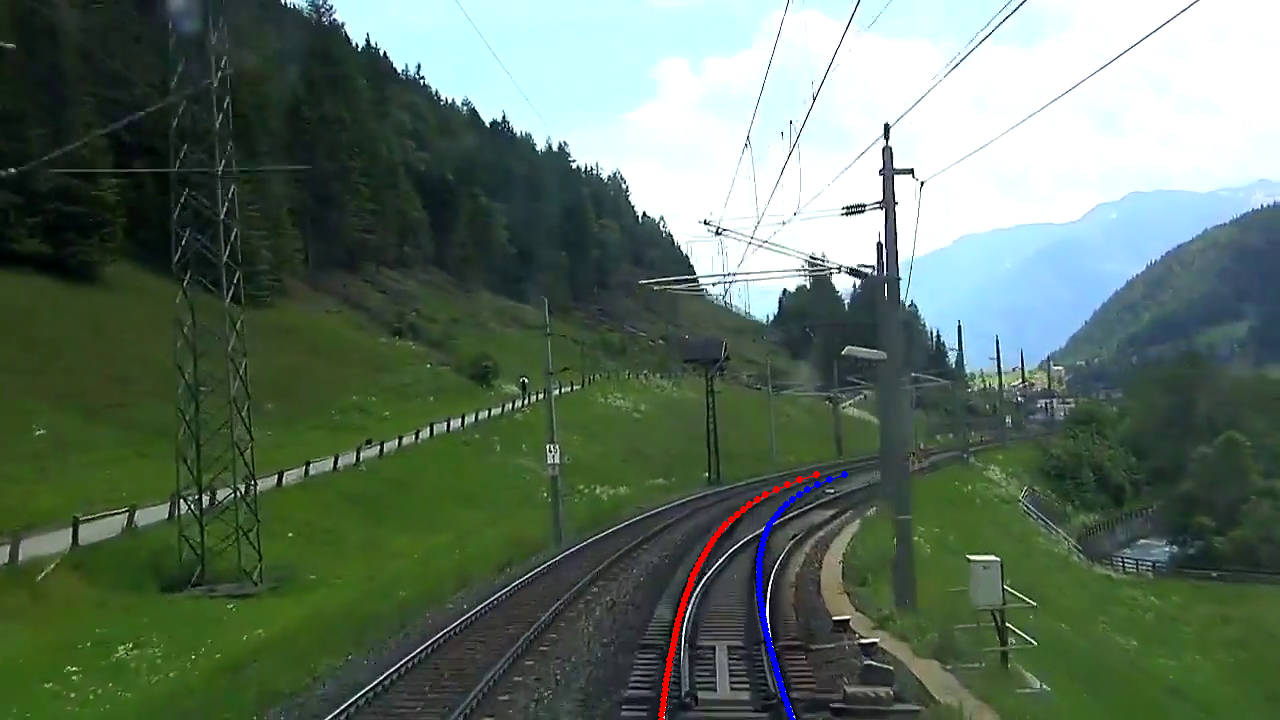
\includegraphics[width=\textwidth]{PICs/experiments/temporalModels/allesRichtig.png}
        \caption{\textbf{Switch 1}: 76/76 frames correct}
        \label{fig:temporalTestSet_a}
    \end{subfigure}
    \hfill
    \begin{subfigure}[b]{0.48\textwidth}
        \centering
        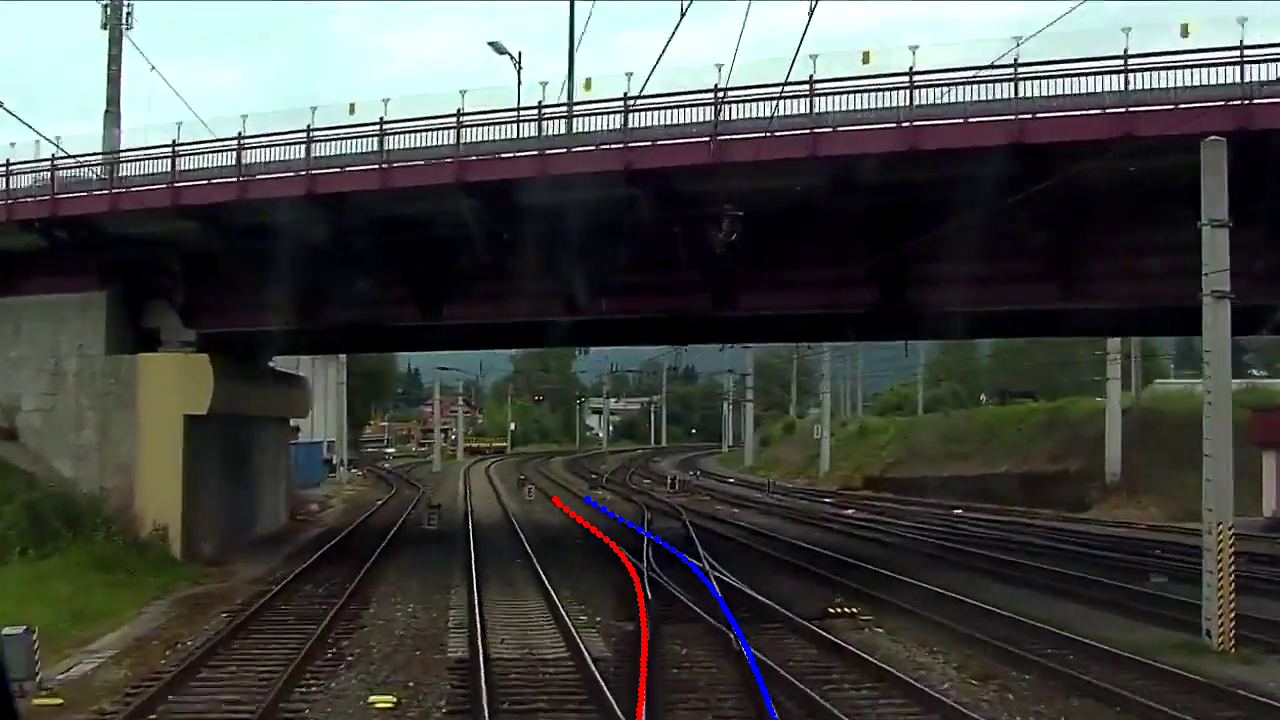
\includegraphics[width=\textwidth]{PICs/experiments/temporalModels/allesFalsch.png}
        \caption{\textbf{Switch 2}: 0/76 frames correct}
    \end{subfigure}
    
    \vspace{0.5cm} % Abstand zwischen den Zeilen

    \begin{subfigure}[b]{0.48\textwidth}
        \centering
        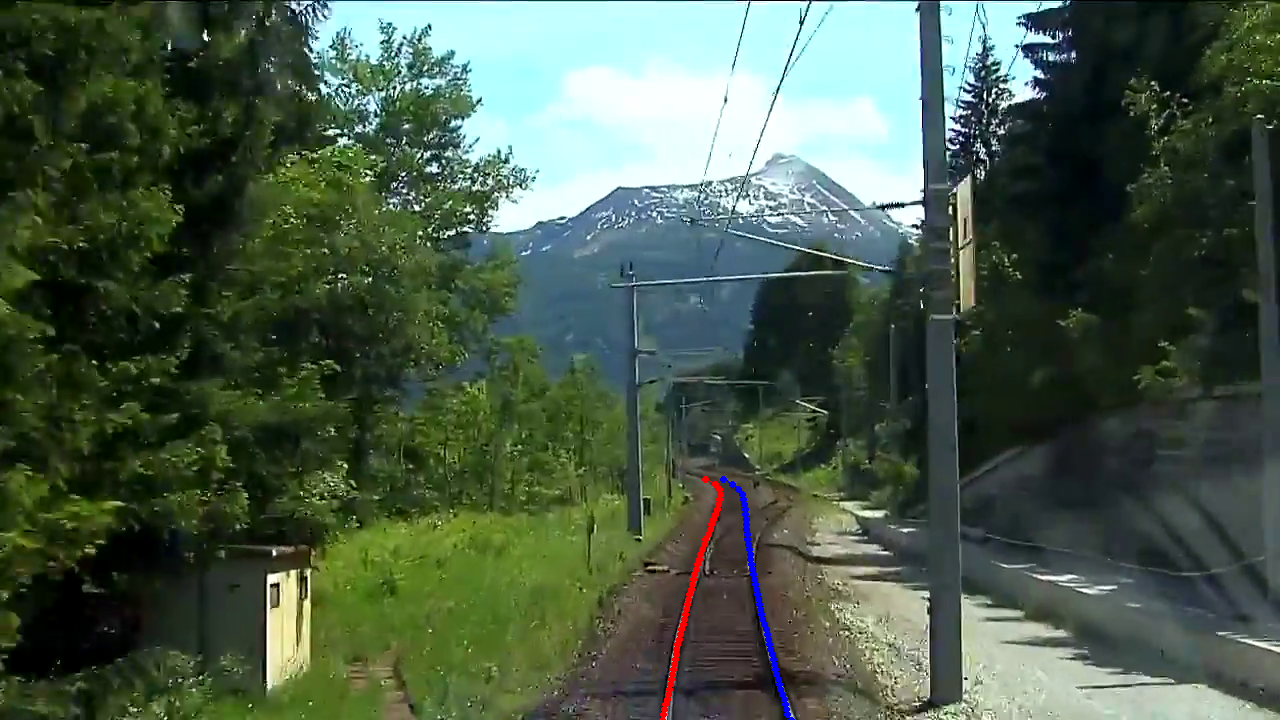
\includegraphics[width=\textwidth]{PICs/experiments/temporalModels/partlyRichtig.png}
        \caption{\textbf{Switch 3}: 36/76 frames correct}
    \end{subfigure}
    \hfill
    \begin{subfigure}[b]{0.48\textwidth}
        \centering
        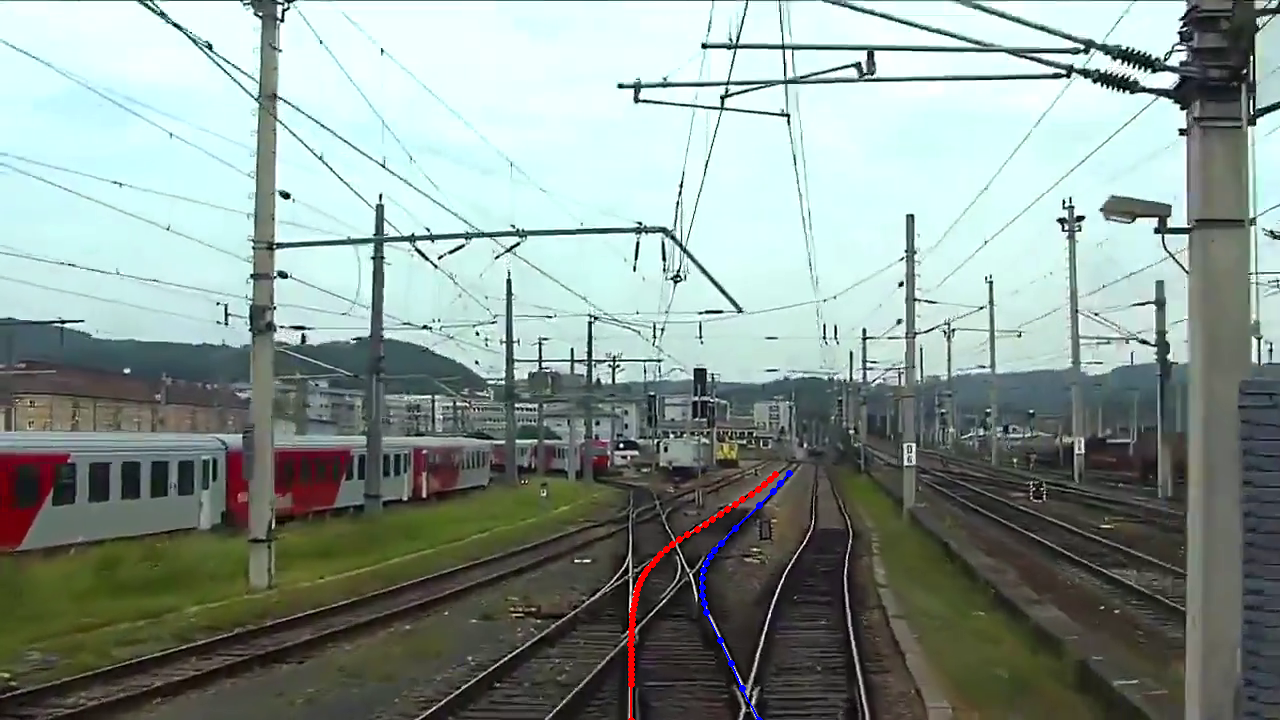
\includegraphics[width=\textwidth]{PICs/experiments/temporalModels/partlyRichtig2.png}
        \caption{\textbf{Switch 4}: 39/76 frames correct}
    \end{subfigure}
    \caption{Temporal test set with annotation. Visualized are the first images of a sequence. The amount of correctly predicted frames from the single-frame-based model.}
    \label{fig:temporalTestSet}
\end{figure}

\subsection{Hyperparameters}

Most experiments, especially the latest ones, are done with the same hyperparameters to provide a fair comparison.
The best-performing single-frame-based model inspires the values used.
That is why the input dimensions are set to $3 \times 512 \times 512$.
Features are extracted with the EfficientNet-B3 backbone in all temporal experiments.
All values for data augmentation, such as color factors, crop margins, or standard deviation factors, are the same.
Furthermore, sequential experiments utilize the Adam optimizer \cite{pytorchAdamOptimizer} and a OneCycle Scheduler \cite{pytorch_oneCycleLR_docu} with the same learning rate parameters.
The best results of single-frame models are obtained with 64 anchors in the output vector.
Therefore, temporal experiments use the same number of anchors.

However, some parameters are altered.
The added complexity of sequential models significantly increases training durations.
Therefore, models train for only 100 epochs in most experiments.
Additionally, the data-handling logic within and before the model sometimes requires a batch size of 1.
Consequently, all different sequential models train with that batch size.

Furthermore, this work adds two hyperparameters to manage sequences and the sliding window.
The sequence length of 76 can be defined if the dataset changes and the window length can be set.
Most experiments use a window length of 10 frames.
\autoref{tab:temporalExperimetparams} describes the most relevant experiments and includes the parameters used.

\vspace{1cm}

\begin{table}[H]
    \centering
    \resizebox{\textwidth}{!}{
    \begin{tabular}{lcccccccccc}
        \hline
        \rowcolor{white} \textbf{Model} & \multicolumn{2}{c}{\textbf{Pre-trained}} & \multicolumn{2}{c}{\textbf{Freezed}} & \multicolumn{3}{c}{\textbf{Data augmentation}} & \textbf{Sliding window} & \textbf{Epochs} & \textbf{Dataset} \\
        \hline
        \rowcolor[gray]{0.9} architecture                & BB & Head (anchors) & BB & Head   & color & flip & crop & length & number & version \\ 
        \hline
        \rowcolor{white}     CNN\_LSTM\_FC               & ENB3 & trapeze (64) & \checkmark &            & \checkmark & \checkmark & \checkmark & 10 & 107 & 1 \\ 
        \rowcolor[gray]{0.9} CNN\_FC\_LSTM               & ENB3 & trapeze (32) & \checkmark & \checkmark & \checkmark & \checkmark & \checkmark & 10 & 400 & 1 \\ 
        \rowcolor{white}     CNN\_LSTM\_V1               & ENB3 &              & \checkmark &            & \checkmark & \checkmark & \checkmark & 10 & 400 & 1 \\
        \rowcolor[gray]{0.9} CNN\_FC\_FCOUT\_V1          & ENB3 & trapeze (64) & \checkmark & \checkmark & \checkmark & \checkmark & \checkmark & 10 & 600 & 1 \\
        \hline
        \rowcolor{white}     CNN\_FC\_LSTM               & ENB3 & trapeze (32) & \checkmark & \checkmark &            & \checkmark & \checkmark & 10 & 400 & 1 \\
        \rowcolor{white}     CNN\_FC\_LSTM               & ENB3 & trapeze (32) & \checkmark & \checkmark &            &            & \checkmark & 10 & 400 & 1 \\
        \rowcolor{white}     CNN\_FC\_LSTM               & ENB3 & trapeze (32) & \checkmark & \checkmark &            &            &            & 10 & 400 & 1 \\
        \rowcolor[gray]{0.9} CNN\_LSTM\_V1               & ENB3 &              & \checkmark &            &            & \checkmark & \checkmark & 10 & 400 & 1 \\
        \rowcolor[gray]{0.9} CNN\_LSTM\_V1               & ENB3 &              & \checkmark &            &            &            & \checkmark & 10 & 400 & 1 \\
        \rowcolor[gray]{0.9} CNN\_LSTM\_V1               & ENB3 &              & \checkmark &            &            &            &            & 10 & 400 & 1 \\
        \rowcolor[gray]{0.9} CNN\_FC\_FCOUT\_V1          & ENB3 & trapeze (64) & \checkmark & \checkmark &            & \checkmark & \checkmark & 10 & 600 & 1 \\
        \rowcolor{white}     CNN\_FC\_FCOUT\_V1          & ENB3 & trapeze (64) & \checkmark & \checkmark &            &            & \checkmark & 10 & 600 & 1 \\
        \hline
        \rowcolor[gray]{0.9} CNN\_FC\_LSTM               & ENB3 & trapeze (32) & \checkmark & \checkmark &            & \checkmark & \checkmark & 30 & 400 & 1 \\
        \rowcolor[gray]{0.9} CNN\_FC\_LSTM               & ENB3 & trapeze (32) & \checkmark & \checkmark &            &            & \checkmark & 30 & 400 & 1 \\
        \rowcolor{white}     CNN\_LSTM\_V1               & ENB3 &              & \checkmark &            &            & \checkmark & \checkmark & 30 & 400 & 1 \\
        \rowcolor{white}     CNN\_LSTM\_V1               & ENB3 &              & \checkmark &            &            &            & \checkmark & 30 & 400 & 1 \\
        \rowcolor[gray]{0.9} CNN\_FC\_FCOUT\_V1          & ENB3 & trapeze (64) & \checkmark & \checkmark &            & \checkmark & \checkmark & 30 & 600 & 1 \\
        \rowcolor[gray]{0.9} CNN\_FC\_FCOUT\_V1          & ENB3 & trapeze (64) & \checkmark & \checkmark &            &            & \checkmark & 30 & 600 & 1 \\
        \hline
        \rowcolor{white}     CNN\_FC\_LSTM               & ENB3 & trapeze (32) & \checkmark & \checkmark &            & \checkmark & \checkmark & 10 & 100 & 2 \\
        \rowcolor[gray]{0.9} CNN\_LSTM\_V1               & ENB3 &              & \checkmark &            &            & \checkmark & \checkmark & 10 & 100 & 2 \\
        \rowcolor{white}     CNN\_FC\_FCOUT\_V1          & ENB3 & trapeze (64) & \checkmark & \checkmark &            & \checkmark & \checkmark & 10 & 100 & 2 \\
        \hline
        \rowcolor[gray]{0.9} CNN\_FC\_LSTM               & ENB3 & trapeze (32) & \checkmark & \checkmark &            &            & \checkmark & 10 & 100 & 3 \\
        \rowcolor{white}     CNN\_LSTM\_V1               & ENB3 &              & \checkmark &            &            &            & \checkmark & 10 & 100 & 3 \\
        \rowcolor[gray]{0.9} CNN\_FC\_FCOUT\_V1          & ENB3 & trapeze (64) & \checkmark & \checkmark &            &            & \checkmark & 10 & 100 & 3 \\
        \rowcolor{white}     CNN\_LSTM\_V2               & ENB3 &              & \checkmark &            &            &            & \checkmark & 10 & 100 & 3 \\
        \rowcolor[gray]{0.9} CNN\_LSTM\_HEAD             & ENB3 & trapeze (64) & \checkmark &            &            &            & \checkmark & 10 & 100 & 3 \\
        \rowcolor{white}     CNN\_FC\_FCOUT\_V2          & ENB3 & trapeze (64) & \checkmark & \checkmark &            &            & \checkmark & 10 & 100 & 3 \\
        \rowcolor[gray]{0.9} CNN\_FLAT\_FC               & ENB3 & trapeze (64) & \checkmark &            &            &            & \checkmark & 10 & 100 & 3 \\
        \rowcolor{white}     CNN\_LSTM\_SKIP\_CAT        & ENB3 & trapeze (32) & \checkmark & \checkmark &            &            & \checkmark & 10 & 100 & 3 \\
        \rowcolor[gray]{0.9} CNN\_LSTM\_SKIP\_MUL\_FRAME & ENB3 & trapeze (32) & \checkmark & \checkmark &            &            & \checkmark & 10 & 100 & 3 \\
        \rowcolor{white}     CNN\_LSTM\_SKIP\_MUL\_TIME  & ENB3 & trapeze (64) & \checkmark & \checkmark &            &            & \checkmark & 10 & 100 & 3 \\
        \hline
        %\rowcolor[gray]{0.9} best with MNV3-Small & xyM & xyB & xyG & xy / xy ms \\
        %\rowcolor{white}     best with MNV3-Large & xyM & xyB & xyG & xy / xy ms \\
        %\hline
    \end{tabular}
    }
    \caption{Chronological progression of temporal experiments including their parameters}
    \label{tab:temporalExperimetparams}
\end{table}

\subsection{Evaluation}

The switch evaluation dataset evaluates the single-frame model's ability to detect tracks in the presence of switches.
This evaluation dataset is needed because the \ac{IoU} is not meaningful when the switch is in the distance, as shown in \autoref{fig:incorrectButHighIoU}.
However, evaluation can now be done on the temporal dataset.
Since the dataset consists of sequences in which a train drives over switches, this switch and the \ac{GT} of the rails are displayed from every possible distance, making the \ac{IoU} more meaningful.

There are different approaches to how temporal models can be evaluated.
All of them are conducted in this work by extensively testing all trained models.
However, the method that resembles a practical application the most is video inference with the auto-cropping mechanism.
Therefore, this evaluation method is implemented and used for this work since it presents the most relevant metrics.
Each test sequence has a lead time of over 500 frames so that crop coordinates can adjust to the situation.
The \ac{IoU} is calculated using the prediction and the \ac{GT} in labeled frames.
This results in a total \ac{IoU} for each sequence and a trend graph that plots the \ac{IoU} of each frame.
Consequently, sequences can be analyzed more thoroughly.
The implemented technique is also used to evaluate the single-frame-based model on the test set of the sequential dataset.
A fair comparison between single-frame and sequence models can be established this way.